% !TeX spellcheck = pl_PL
%%%%%%%%%%%%%%%%%%%%%%%%%%%%%%%%%%%%%%%%%%%
%                                        %
% Szablon pracy dyplomowej inzynierskiej %
% zgodny  z aktualnymi  przepisami  SZJK %
%                                        %
%%%%%%%%%%%%%%%%%%%%%%%%%%%%%%%%%%%%%%%%%%
%                                        %
%  (c) Krzysztof Simiński, 2018-2023     %
%                                        %
%%%%%%%%%%%%%%%%%%%%%%%%%%%%%%%%%%%%%%%%%%
%                                        %
% Najnowsza wersja szablonów jest        %
% podstępna pod adresem                  %
% github.com/ksiminski/polsl-aei-theses  %
%                                        %
%%%%%%%%%%%%%%%%%%%%%%%%%%%%%%%%%%%%%%%%%%
%
%
% Projekt LaTeXowy zapewnia odpowiednie formatowanie pracy,
% zgodnie z wymaganiami Systemu zapewniania jakości kształcenia.
% Proszę nie zmieniać ustawień formatowania (np. fontu,
% marginesów, wytłuszczeń, kursywy itd. ).
%
% Projekt można kompilować na kilka sposobów.
%
% 1. kompilacja pdfLaTeX
%
% pdflatex main
% bibtex   main
% pdflatex main
% pdflatex main
%
%
% 2. kompilacja XeLaTeX
%
% Kompilatacja przy użyciu XeLaTeXa różni się tym, że na stronie
% tytułowej używany jest font Calibri. Wymaga to jego uprzedniego
% zainstalowania.
%
% xelatex main
% bibtex  main
% xelatex main
% xelatex main
%
%
%%%%%%%%%%%%%%%%%%%%%%%%%%%%%%%%%%%%%%%%%%%%%%%%%%%%%
% W przypadku pytań, uwag, proszę pisać na adres:   %
%      krzysztof.siminski(małpa)polsl.pl            %
%%%%%%%%%%%%%%%%%%%%%%%%%%%%%%%%%%%%%%%%%%%%%%%%%%%%%
%
% Chcemy ulepszać szablony LaTeXowe prac dyplomowych.
% Wypełniając ankietę spod poniższego adresu pomogą
% Państwo nam to zrobić. Ankieta jest całkowicie
% anonimowa. Dziękujemy!


% https://docs.google.com/forms/d/e/1FAIpQLScyllVxNKzKFHfILDfdbwC-jvT8YL0RSTFs-s27UGw9CKn-fQ/viewform?usp=sf_link
%
%%%%%%%%%%%%%%%%%%%%%%%%%%%%%%%%%%%%%%%%%%%%%%%%%%%%%%%%%%%%%%%%%%%%%%%%%

%%%%%%%%%%%%%%%%%%%%%%%%%%%%%%%%%%%%%%%%%%%%%%%
%                                             %
% PERSONALIZACJA PRACY – DANE PRACY           %
%                                             %
%%%%%%%%%%%%%%%%%%%%%%%%%%%%%%%%%%%%%%%%%%%%%%%

% Proszę wpisać swoje dane w poniższych definicjach.

% TODO
% dane autora
\newcommand{\FirstNameAuthor}{Imię}
\newcommand{\SurnameAuthor}{Nazwisko}
\newcommand{\IdAuthor}{$\langle$wpisać właściwy$\rangle$}   % numer albumu  (bez $\langle$ i $\rangle$)

% drugi autor:
%\newcommand{\FirstNameCoauthor}{Imię}   % Jeżeli jest drugi autor, to tutaj należy podać imię.
%\newcommand{\SurnameCoauthor}{Nazwisko} % Jeżeli jest drugi autor, to tutaj należy podać nazwisko.
%\newcommand{\IdCoauthor}{$\langle$wpisać właściwy$\rangle$}  % numer albumu drugiego autora (bez $\langle$ i $\rangle$)
% Gdy nie ma drugiego autora, należy zostawić poniższe definicje puste, jak poniżej. Gdy jest drugi autor, należy zakomentować te linie.
\newcommand{\FirstNameCoauthor}{} % Jeżeli praca ma tylko jednego autora, to dane drugiego autora zostają puste.
\newcommand{\SurnameCoauthor}{}   % Jeżeli praca ma tylko jednego autora, to dane drugiego autora zostają puste.
\newcommand{\IdCoauthor}{}  % Jeżeli praca ma tylko jednego autora, to dane drugiego autora zostają puste.
%%%%%%%%%%

\newcommand{\Supervisor}{$\langle$tytuł lub stopień naukowy oraz imię i nazwisko$\rangle$}     % dane promotora (bez $\langle$ i $\rangle$)
\newcommand{\Title}{Tytuł pracy dyplomowej inżynierskiej}           % tytuł pracy po polsku
\newcommand{\TitleAlt}{Thesis title in English}                     % thesis title in English
\newcommand{\Program}{$\langle$wpisać właściwy$\rangle$}            % kierunek studiów  (bez $\langle$ i $\rangle$)
\newcommand{\Specialisation}{$\langle$wpisać właściwą$\rangle$}     % specjalność  (bez $\langle$ i $\rangle$)
\newcommand{\Departament}{$\langle$wpisać właściwą$\rangle$}        % katedra promotora  (bez $\langle$ i $\rangle$)

% Jeżeli został wyznaczony promotor pomocniczy lub opiekun, proszę go/ją wpisać ...
\newcommand{\Consultant}{$\langle$stopień naukowy imię i nazwisko$\rangle$} % dane promotora pomocniczego, opiekuna (bez $\langle$ i $\rangle$)
% ... w przeciwnym razie proszę zostawić puste miejsce jak poniżej:
%\newcommand{\Consultant}{} % brak promotowa pomocniczego / opiekuna

% koniec fragmentu do modyfikacji
%%%%%%%%%%%%%%%%%%%%%%%%%%%%%%%%%%%%%%%%%%


%%%%%%%%%%%%%%%%%%%%%%%%%%%%%%%%%%%%%%%%%%%%%%%
%                                             %
% KONIEC PERSONALIZACJI PRACY                 %
%                                             %
%%%%%%%%%%%%%%%%%%%%%%%%%%%%%%%%%%%%%%%%%%%%%%%

%%%%%%%%%%%%%%%%%%%%%%%%%%%%%%%%%%%%%%%%


%%%%%%%%%%%%%%%%%%%%%%%%%%%%%%%%%%%%%%%%%%%%%%%
%                                             %
% PROSZĘ NIE MODYFIKOWAĆ PONIŻSZYCH USTAWIEŃ! %
%                                             %
%%%%%%%%%%%%%%%%%%%%%%%%%%%%%%%%%%%%%%%%%%%%%%%



\documentclass[a4paper,twoside,12pt]{book}
\usepackage[utf8]{inputenc}                                      
\usepackage[T1]{fontenc}  
\usepackage{amsmath,amsfonts,amssymb,amsthm}
\usepackage[british,polish]{babel} 
\usepackage{indentfirst}
\usepackage{xurl}
\usepackage{xstring}
\usepackage{ifthen}



\usepackage{ifxetex}

\ifxetex
	\usepackage{fontspec}
	\defaultfontfeatures{Mapping=tex—text} % to support TeX conventions like ``——-''
	\usepackage{xunicode} % Unicode support for LaTeX character names (accents, European chars, etc)
	\usepackage{xltxtra} % Extra customizations for XeLaTeX
\else
	\usepackage{lmodern}
\fi



\usepackage[margin=2.5cm]{geometry}
\usepackage{graphicx} 
\usepackage{hyperref}
\usepackage{booktabs}
\usepackage{tikz}
\usepackage{pgfplots}
\usepackage{mathtools}
\usepackage{geometry}
\usepackage{subcaption}   % subfigures
\usepackage[page]{appendix} % toc,
\renewcommand{\appendixtocname}{Dodatki}
\renewcommand{\appendixpagename}{Dodatki}
\renewcommand{\appendixname}{Dodatek}

\usepackage{csquotes}
\usepackage[natbib=true,backend=bibtex,maxbibnames=99]{biblatex}  % kompilacja bibliografii BibTeXem
%\usepackage[natbib=true,backend=biber,maxbibnames=99]{biblatex}  % kompilacja bibliografii Biberem
\bibliography{biblio}

\usepackage{ifmtarg}   % empty commands  

\usepackage{setspace}
\onehalfspacing


\frenchspacing

%%%%%%%%%%%%%%%%%%%%%%%%%%%%%%%%%%
% środowiska dla definicji, twierdzenia, przykładu
\usepackage{amsthm}

\newtheorem{Definition}{Definicja}
\newtheorem{Example}{Przykład}
\newtheorem{Theorem}{Twierdzenie}
%%%%%%%%%%%%%%%%%%%%%%%%%%%%%%%%%%

%%%% TODO LIST GENERATOR %%%%%%%%%

\usepackage{color}
\definecolor{brickred}      {cmyk}{0   , 0.89, 0.94, 0.28}

\makeatletter \newcommand \kslistofremarks{\section*{Uwagi} \@starttoc{rks}}
  \newcommand\l@uwagas[2]
    {\par\noindent \textbf{#2:} %\parbox{10cm}
{#1}\par} \makeatother


\newcommand{\ksremark}[1]{%
{%\marginpar{\textdbend}
{\color{brickred}{[#1]}}}%
\addcontentsline{rks}{uwagas}{\protect{#1}}%
}

\newcommand{\comma}{\ksremark{przecinek}}
\newcommand{\nocomma}{\ksremark{bez przecinka}}
\newcommand{\styl}{\ksremark{styl}}
\newcommand{\ortografia}{\ksremark{ortografia}}
\newcommand{\fleksja}{\ksremark{fleksja}}
\newcommand{\pauza}{\ksremark{pauza `--', nie dywiz `-'}}
\newcommand{\kolokwializm}{\ksremark{kolokwializm}}
\newcommand{\cudzyslowy}{\ksremark{\,\,polskie cudzysłowy''}}

%%%%%%%%%%%%%% END OF TODO LIST GENERATOR %%%%%%%%%%%

\newcommand{\printCoauthor}{%		
    \StrLen{\FirstNameCoauthor}[\FNCoALen]
    \ifthenelse{\FNCoALen > 0}%
    {%
		{\large\bfseries\Coauthor\par}
	
		{\normalsize\bfseries \LeftId: \IdCoauthor\par}
    }%
    {}
} 

%%%%%%%%%%%%%%%%%%%%%
\newcommand{\autor}{%		
    \StrLen{\FirstNameCoauthor}[\FNCoALenXX]
    \ifthenelse{\FNCoALenXX > 0}%
    {\FirstNameAuthor\ \SurnameAuthor, \FirstNameCoauthor\ \SurnameCoauthor}%
	{\FirstNameAuthor\ \SurnameAuthor}%
}
%%%%%%%%%%%%%%%%%%%%%

\StrLen{\FirstNameCoauthor}[\FNCoALen]
\ifthenelse{\FNCoALen > 0}%
{%
\author{\FirstNameAuthor\ \SurnameAuthor, \FirstNameCoauthor\ \SurnameCoauthor}
}%
{%
\author{\FirstNameAuthor\ \SurnameAuthor}
}%

%%%%%%%%%%%% ZYWA PAGINA %%%%%%%%%%%%%%%
% brak kapitalizacji zywej paginy
\usepackage{fancyhdr}
\pagestyle{fancy}
\fancyhf{}
\fancyhead[LO]{\nouppercase{\it\rightmark}}
\fancyhead[RE]{\nouppercase{\it\leftmark}}
\fancyhead[LE,RO]{\it\thepage}


\fancypagestyle{tylkoNumeryStron}{%
   \fancyhf{} 
   \fancyhead[LE,RO]{\it\thepage}
}

\fancypagestyle{bezNumeracji}{%
   \fancyhf{} 
   \fancyhead[LE,RO]{}
}


\fancypagestyle{NumeryStronNazwyRozdzialow}{%
   \fancyhf{} 
   \fancyhead[LE]{\nouppercase{\autor}}
   \fancyhead[RO]{\nouppercase{\leftmark}} 
   \fancyfoot[CE, CO]{\thepage}
}


%%%%%%%%%%%%% OBCE WTRETY  
\newcommand{\obcy}[1]{\emph{#1}}
\newcommand{\english}[1]{{\selectlanguage{british}\obcy{#1}}}
%%%%%%%%%%%%%%%%%%%%%%%%%%%%%

% polskie oznaczenia funkcji matematycznych
\renewcommand{\tan}{\operatorname {tg}}
\renewcommand{\log}{\operatorname {lg}}

% jeszcze jakies drobiazgi

\newcounter{stronyPozaNumeracja}

%%%%%%%%%%%%%%%%%%%%%%%%%%% 
\newcommand{\printOpiekun}[1]{%		

    \StrLen{\Consultant}[\mystringlen]
    \ifthenelse{\mystringlen > 0}%
    {%
       {\large{\bfseries OPIEKUN, PROMOTOR POMOCNICZY}\par}
       
       {\large{\bfseries \Consultant}\par}
    }%
    {}
} 
%
%%%%%%%%%%%%%%%%%%%%%%%%%%%%%%%%%%%%%%%%%%%%%%
 
% Proszę nie modyfikować poniższych definicji!
\newcommand{\Author}{\FirstNameAuthor\ \MakeUppercase{\SurnameAuthor}} 
\newcommand{\Coauthor}{\FirstNameCoauthor\ \MakeUppercase{\SurnameCoauthor}}
\newcommand{\Type}{PROJEKT INŻYNIERSKI}
\newcommand{\Faculty}{Wydział Automatyki, Elektroniki i Informatyki} 
\newcommand{\Polsl}{Politechnika Śląska}
\newcommand{\Logo}{politechnika_sl_logo_bw_pion_pl.pdf}
\newcommand{\LeftId}{Nr albumu}
\newcommand{\LeftProgram}{Kierunek}
\newcommand{\LeftSpecialisation}{Specjalność}
\newcommand{\LeftSUPERVISOR}{PROWADZĄCY PRACĘ}
\newcommand{\LeftDEPARTMENT}{KATEDRA}
%%%%%%%%%%%%%%%%%%%%%%%%%%%%%%%%%%%%%%%%%%%%%%

%%%%%%%%%%%%%%%%%%%%%%%%%%%%%%%%%%%%%%%%%%%%%%%
%                                             %
% KONIEC USTAWIEŃ                             %
%                                             %
%%%%%%%%%%%%%%%%%%%%%%%%%%%%%%%%%%%%%%%%%%%%%%%




%%%%%%%%%%%%%%%%%%%%%%%%%%%%%%%%%%%%%%%%%%%%%%%
%                                             %
% MOJE PAKIETY, USTAWIENIA ITD                %
%                                             %
%%%%%%%%%%%%%%%%%%%%%%%%%%%%%%%%%%%%%%%%%%%%%%%

% Tutaj proszę umieszczać swoje pakiety, makra, ustawienia itd.


 
%%%%%%%%%%%%%%%%%%%%%%%%%%%%%%%%%%%%%%%%%%%%%%%%%%%%%%%%%%%%%%%%%%%%%
% listingi i fragmentu kodu źródłowego 
% pakiet: listings lub minted
% % % % % % % % % % % % % % % % % % % % % % % % % % % % % % % % % % % 

% biblioteka listings
\usepackage{listings}
\lstset{%
morekeywords={string,exception,std,vector},% słowa kluczowe rozpoznawane przez pakiet listings
language=C++,% C, Matlab, Python, SQL, TeX, XML, bash, ... – vide https://www.ctan.org/pkg/listings
commentstyle=\textit,%
identifierstyle=\textsf,%
keywordstyle=\sffamily\bfseries, %\texttt, %
%captionpos=b,%
tabsize=3,%
frame=lines,%
numbers=left,%
numberstyle=\tiny,%
numbersep=5pt,%
breaklines=true,%
escapeinside={@*}{*@},%
}

% % % % % % % % % % % % % % % % % % % % % % % % % % % % % % % % % % % 
% pakiet minted
%\usepackage{minted}

% pakiet wymaga specjalnego kompilowania:
% pdflatex -shell-escape main.tex
% xelatex  -shell-escape main.tex

%\usepackage[chapter]{minted} % [section]
%%\usemintedstyle{bw}   % czarno-białe kody 
%
%\setminted % https://ctan.org/pkg/minted
%{
%%fontsize=\normalsize,%\footnotesize,
%%captionpos=b,%
%tabsize=3,%
%frame=lines,%
%framesep=2mm,
%numbers=left,%
%numbersep=5pt,%
%breaklines=true,%
%escapeinside=@@,%
%}

%%%%%%%%%%%%%%%%%%%%%%%%%%%%%%%%%%%%%%%%%%%%%%%%%%%%%%%%%%%%%%%%%%%%%



%%%%%%%%%%%%%%%%%%%%%%%%%%%%%%%%%%%%%%%%%%%%%%%
%                                             %
% KONIEC MOICH USTAWIEŃ                       %
%                                             %
%%%%%%%%%%%%%%%%%%%%%%%%%%%%%%%%%%%%%%%%%%%%%%%



%%%%%%%%%%%%%%%%%%%%%%%%%%%%%%%%%%%%%%%%


\begin{document}
%\kslistofremarks

\frontmatter

%%%%%%%%%%%%%%%%%%%%%%%%%%%%%%%%%%%%%%%%%%%%%%%
%                                             %
% PROSZĘ NIE MODYFIKOWAĆ STRONY TYTUŁOWEJ!    %
%                                             %
%%%%%%%%%%%%%%%%%%%%%%%%%%%%%%%%%%%%%%%%%%%%%%%


%%%%%%%%%%%%%%%%%%  STRONA TYTUŁOWA %%%%%%%%%%%%%%%%%%%
\pagestyle{empty}
{
	\newgeometry{top=1.5cm,%
	             bottom=2.5cm,%
	             left=3cm,
	             right=2.5cm}
 
	\ifxetex 
	  \begingroup
	  \setsansfont{Calibri}
	   
	\fi 
	 \sffamily
	\begin{center}
	\includegraphics[width=50mm]{\Logo}
	 
	
	{\Large\bfseries\Type\par}
	
	\vfill  \vfill  
			 
	{\large\Title\par}
	
	\vfill  
		
	{\large\bfseries\Author\par}
	
	{\normalsize\bfseries \LeftId: \IdAuthor}

	\printCoauthor
	
	\vfill  		
 
	{\large{\bfseries \LeftProgram:} \Program\par} 
	
	{\large{\bfseries \LeftSpecialisation:} \Specialisation\par} 
	 		
	\vfill  \vfill 	\vfill 	\vfill 	\vfill 	\vfill 	\vfill  
	 
	{\large{\bfseries \LeftSUPERVISOR}\par}
	
	{\large{\bfseries \Supervisor}\par}
				
	{\large{\bfseries \LeftDEPARTMENT\ \Departament} \par}
		
	{\large{\bfseries \Faculty}\par}
		
	\vfill  \vfill  

    	
    \printOpiekun{\Consultant}
    
	\vfill  \vfill  
		
    {\large\bfseries  Gliwice \the\year}

   \end{center}	
       \ifxetex 
       	  \endgroup
       \fi
	\restoregeometry
}
  
%%%%%%%%%%%%%%%%%%%%%%%%%%%%%%%%%%%%%%%%%%%%%%%
%                                             %
% KONIEC STRONY TYTUŁOWEJ                     %
%                                             %
%%%%%%%%%%%%%%%%%%%%%%%%%%%%%%%%%%%%%%%%%%%%%%%  


\cleardoublepage

\rmfamily\normalfont
\pagestyle{empty}


%%% No to zaczynamy pisać pracę :-) %%%%

% TODO
\subsubsection*{Tytuł pracy} 
\Title

\subsubsection*{Streszczenie}  
(Streszczenie pracy – odpowiednie pole w systemie APD powinno zawierać kopię tego streszczenia.)

\subsubsection*{Słowa kluczowe} 
(2-5 slow (fraz) kluczowych, oddzielonych przecinkami)

\subsubsection*{Thesis title} 
\begin{otherlanguage}{british}
\TitleAlt
\end{otherlanguage}

\subsubsection*{Abstract} 
\begin{otherlanguage}{british}
(Thesis abstract – to be copied into an appropriate field during an electronic submission – in English.)
\end{otherlanguage}
\subsubsection*{Key words}  
\begin{otherlanguage}{british}
(2-5 keywords, separated by commas)
\end{otherlanguage}

%%%%%%%%%%%%%%%%%% SPIS TRESCI %%%%%%%%%%%%%%%%%%%%%%
% Add \thispagestyle{empty} to the toc file (main.toc), because \pagestyle{empty} doesn't work if the TOC has multiple pages
\addtocontents{toc}{\protect\thispagestyle{empty}}
\tableofcontents

%%%%%%%%%%%%%%%%%%%%%%%%%%%%%%%%%%%%%%%%%%%%%%%%%%%%%
\setcounter{stronyPozaNumeracja}{\value{page}}
\mainmatter
\pagestyle{empty}

\cleardoublepage

\pagestyle{NumeryStronNazwyRozdzialow}

%%%%%%%%%%%%%% wlasciwa tresc pracy %%%%%%%%%%%%%%%%%

%%%%%%%%%%%%%% rozdział 1 - wstęp %%%%%%%%%%%%%%%%%
\chapter{Wstęp}
\label{ch:wstep}

Robotyka to obszar badawczy i techniczny poświęcony teorii, konstrukcji oraz praktycznym zastosowaniom robotów. Elementami wykonawczymi układów zrobotyzowanych są najczęściej silniki lub siłowniki, te drugie nierzadko napędzane wewnętrznie silnikami. Silnik jest rodzajem maszyny zamieniającym jeden rodzaj energii --- w robotyce najczęściej elektryczną --- na energię mechaniczną, czego celem jest wprawienie w ruch elementów ruchomych.

W przypadku prostych układów, takich jak podajnik taśmowy napędzany pojedynczym silnikiem, precyzja sterowania nie ma wysokiego priorytetu. Najważniejsze jest, by element znajdujący się na taśmie przejechał z punktu A do punktu B z pewną prędkością, a jego położeniem zajmą się inne czujniki. Jednak gdy silnik napędza ramię robota, pojazd lub drona, ważne jest, by utrzymywał stałą prędkość i/lub wykonywał określoną ilość obrotów.

Z tego powodu, jednym z wyzwań, z jakimi mierzyli się pionierzy automatycy-robotycy jest precyzyjne sterowanie tworzonymi przez siebie układami. Jest to kwestia o tyle istotna, że gdy odpowiedź układu odbiega --- nawet w niewielkim stopniu --- od wartości zadanej, staje się on znacząco trudniejszy w użytkowaniu (sterowaniu), a w skrajnych przypadkach bezużyteczny.

Jako rozwiązanie tego problemu, powstał poddział robotyki zwany odometrią. Jest to dział na pograniczu robotyki i miernictwa, zajmujący się użyciem różnego rodzaju czujników w celu oszacowania położenia ruchomego układu względem pozycji startowej w przestrzeni fizycznej.

Współcześni automatycy-robotycy będący na początku swojej ścieżki edukacji/kariery, lub zajmujący się nią jedynie hobbystycznie, również mierzą się prędzej czy później z problemem precyzji sterowania układu.

%%%%%%%%%%%%%% rozdział 2 - analiza %%%%%%%%%%%%%%%%%
\chapter{[Analiza tematu]}
Problem synchronizowania silników elektrycznych znany jest w~dziedzinie automatyki od dziesiątek lat. Początki badania silników sięgają XIX wieku, kiedy to Michael Faraday oraz inni naukowcy eksperymentowali ze wykorzystaniem elektromagnetyzmu\cite{bib:pierwszesilniki}. Pierwsze silniki elektryczne były prymitywne i~nie miały zaawansowanych metod sterowania. Wczesne próby pozycjonowania opierały się głównie na prostych mechanizmach, takich jak przekładnie i~sprzęgła.

W miarę postępu technologicznego, szczególnie w~XX wieku, rozwijano bardziej zaawansowane metody pozycjonowania. Pojawiły się pierwsze systemy sterowania, wykorzystujące technologię zwrotną informacji, mającą na celu monitorowanie i~regulację położenia wałów silników. Jednak precyzja tych rozwiązań była ograniczona, a~dokładność pozycjonowania nie zawsze spełniała wymagania coraz bardziej zaawansowanych zastosowań.

Dopiero wprowadzenie enkoderów (Definicja~\ref{def:enkoder}) elektronicznych w~latach 60.~XX~wieku\cite{bib:pierwszeenkodery} stało się przełomem.

\begin{Definition}[Enkoder obrotowy]\label{def:enkoder}
    Urządzenie, generujące sygnały elektryczne odpowiadające ruchowi obrotowemu wału silnika celem określenia jego pozycji. 
\end{Definition}

Początkowo enkodery były oparte na szczotkach stykających się z dyskiem zawierającym serię odpowiednio zakodowanych pierścieni koncentrycznych (Rysunek~\ref{fig:encoderDiscAbsolute}), wypełnionych otworami o odpowiedniej długości\cite{bib:rodzajeenkoderow}. Są one tanie w~produkcji, jednak mają swoje ograniczenia związane ze zużyciem mechanicznym elementów stykowych, niską maksymalną dozwoloną prędkością silnika i~wymaganiami konserwacji. Ten typ enkoderów spotykany jest do dziś, na przykład w multimetrach cyfrowych.

Rozwój technologii przyniósł enkodery optyczne, wykorzystujące diody LED i~fotodetektory. Później pojawiły się enkodery magnetyczne. To właśnie one --- enkodery optyczne i~magnetyczne --- są do dnia dzisiejszego najczęściej spotykane i~oferują najwyższą dokładność sterowania przy niskich kosztach i~niewielkim stopniu skomplikowania. To właśnie na nich skupiono się w~dalszej części pracy.

Enkodery można podzielić ze względu na\cite{bib:rodzajeenkoderow}:
\begin{itemize}
    \item Metodę używaną do odczytania pozycji: kontaktowe i~bezkontaktowe.
    \item Rodzaj sygnału wyjściowego: pozycja absolutna lub szereg inkrementujących/dekrementujących wartości.
    \item Zjawisko fizyczne wykorzystane do przesłania sygnału pozycyjnego: przewodzenie elektryczne, magnetyzm, zjawiska optyczne lub pojemnościowe.
\end{itemize}

Najważniejszy jest podział ze względu na rodzaj sygnału wyjściowego. Mimo, że zarówno enkodery absolutne jak i~inkrementalne posiadają dyski kodujące, różnią się one działaniem. Enkodery absolutne jako sygnał wyjściowy podają precyzyjną pozycję wału silnika, najczęściej zakodowaną w~słowie bitowym. Przykładowy wygląd dysku kodującego widoczny jest na Rysunku~\ref{fig:encoderDiscAbsolute}. Istotną cechą tego rodzaju enkoderów jest możliwość określenia pozycji nawet po utracie zasilania.

\begin{center}
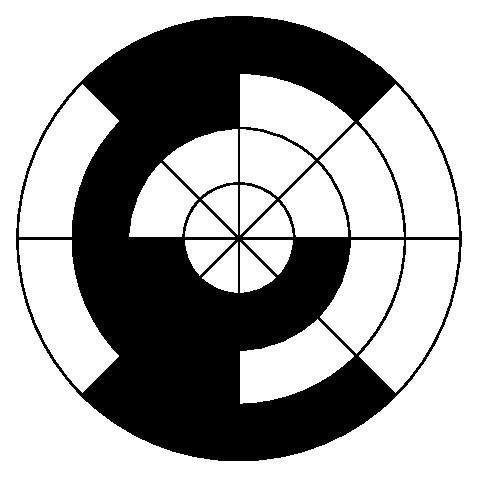
\includegraphics[scale=1]{images/encoderDiscAbsolute.eps}
\captionof{figure}{Poglądowy schemat dysku enkodera absolutnego z 3-bitowym kodem Graya\cite{bib:tarczaenkoderaabsolutnego}.}
\label{fig:encoderDiscAbsolute}
\end{center}

Enkodery inkrementalne u~podstaw działają~w ten sam sposób, tzn. opierają się na dyskach kodujących, z~tą różnicą, że nie są w~stanie podać dokładnej wartości położenia. Zamiast tego, podają na wyjściu odpowiedni impuls przy obrocie w~danym kierunku. Następnie w~oprogramowaniu impulsy te są zliczane w celu oszacowania aktualnej pozycji względem pozycji startowej. Ze względu na wyzerowanie liczby impulsów przy utracie zasilania, ten typ enkodera nie jest w~stanie podać dokładnej pozycji w~przypadku utraty zasilania.

Istotny jest również podział enkoderów ze względu na wykorzystywane zjawisko fizyczne. Dwa główne typy to enkodery optyczne oraz magnetyczne. Pierwszy rodzaj występuje zarówno w~wariancie pojedynczym (Rysunek~\ref{fig:encoderDiscIncrementalSingle}) jak i~podwójnym (Rysunek~\ref{fig:encoderDiscIncrementalDual}). Drugi zaś, ze względu na występowanie polaryzacji biegunów, jedynie w~wariancie pojedynczym (Rysunek~\ref{fig:encoderDiscIncrementalSingle}). W~przypadku enkoderów optycznych, kolorowi białemu odpowiada szczelina, zaś kolorowi czarnemu blokada. W~przypadku enkoderów optycznych, kolorom odopowiadają bieguny~S~i~N.

\begin{figure}
    \centering
    \subfloat[Enkoder pojedynczy]{
      
\includegraphics[width=6cm]{images/encoderDiscIncrementalSingle.eps}
      \label{fig:encoderDiscIncrementalSingle}
    }\qquad
    \subfloat[Enkoder podwójny (kwadratowy)]{
      
\includegraphics[width=6cm]{images/encoderDiscIncrementalDual.eps}
      \label{fig:encoderDiscIncrementalDual}
    }
    \caption{Poglądowe schematy dysku enkodera inkrementalnego \cite{bib:tarczeenkoderowinkrementalnych}}
\end{figure}

%%%%%%%%%%%%%% rozdział 3 - wymagania i narzędzia %%%%%%%%%%%%%%%%%
\chapter{Wymagania i narzędzia}
\section{Założenia i narzędzia}
\label{ch:zalozenia}
Założenia podzielone zostały na kilka podsekcji, po jednej dla każdej części projektu. Wyjaśnienie poszczególnych części/modułów znajduje się w Rozdziale \ref{ch:project}.

\subsection*{Założenia dla układu elektronicznego}
\begin{itemize}
    \item 2 silniki DC (ang.~\english{Direct Current})
    \item sterownik silników
    \item czujnik laserowy z przodu pojazdu
    \item enkodery optyczne do pomiaru położenia wałów silników
    \item sterowanie przy użyciu mikroprocesora
    \item LED (ang.~\english{Light Emitting Diode}) sygnalizujący stan oprogramowania mikroprocesora
    \item głośnik sygnalizujący stan oprogramowania mikroprocesora
    \item bezpieczniki zabezpieczające układ elektroniczny
    \item przełączniki źródeł prądowych
\end{itemize}

\subsection*{Założenia dla modelu pojazdu}
\begin{itemize}
    \item 4 koła
    \item możliwa jazda do przodu, tyłu oraz skręcanie jak w samochodzie osobowym
    \item kilka rozmiarów kół dla różnorodności eksperymentalnej
    \item modułowość pozwalająca na modyfikację w razie potrzeby
    \item projekt wizualny podobny do samochodu osobowego
    \item w miarę możliwości niska masa
    \item obudowa wydrukowana na drukarce 3D
\end{itemize}

\subsection*{Założenia dla oprogramowania mikroprocesora}
\begin{itemize}
    \item system FreeRTOS (ang.~\english{Real Time Operating System})
    \item wykonanie w języku C++
    \item klient UDP (ang.~\english{User Datagram Protocol})
    \item serwer UDP
    \item interpretacja danych z ramek pakietów UDP
    \item sterowanie możliwe w układzie otwartym lub zamkniętym
    \item wartość zadana odbierana z aplikacji mobilnej przez wifi
    \item rozpoczęcie i zakończenie pomiaru na komendę z aplikacji mobilnej
    \item awaryjne zakończenie pomiaru w przypadku rozłączenia wifi
    \item odczytywanie kierunku i położenia enkoderów
    \item synchronizacja silników
    \item obliczanie sygnałów sterujących silników
    \item regulatory PID
    \item plik konfiguracyjny
\end{itemize}

\subsection*{Założenia dla aplikacji mobilnej}
\begin{itemize}
    \item działanie na systemie Android
    \item prostota wykonania
    \item prostota użytkowania
    \item krótki czas tworzenia (ang.~\english{development})
    \item klient UDP
    \item serwer UDP
    \item interpretacja danych z ramek pakietów UDP
    \item zmienny docelowy adres IP (ang.~\english{Internet Protocol}) 
    \item parametryzacja regulatorów PID
    \item ustawianie wartości zadanej
    \item ustawianie prędkości
\end{itemize}

\subsection*{Założenia dla skryptu odbierającego dane}
\begin{itemize}
    \item działanie na systemie windows
    \item wykonanie w języku Python
    \item serwer UDP
    \item interpretacja danych z ramek pakietów UDP
    \item zapis danych do pliku .csv (ang.~\english{Comma-Separated Values})
    \item działanie w pętli; możliwość odbioru wielu pomiarów
\end{itemize}

\subsection*{Założenia dla skryptu wizualizujacego dane}
\begin{itemize}
    \item działanie na systemie windows
    \item odczytywanie danych z pliku .csv
    \item wizualizacja odczytanych danych (tworzenie wykresów)
    \item zapisywanie wykresów do pliku .eps (ang.~\english{Encapsulated PostScript})
\end{itemize}

\newpage

\section{Narzędzia}
\label{ch:narzedzia}
% ============ hardware ============ %
\subsection*{Narzędzia fizyczne}

\subsubsection*{Zestaw lutowniczy} % kim był Transformatorov?
Lutowanie to proces łączenia elementów elektronicznych przez stopienie spoiwa lutowniczego na przylegających do siebie elementach metalowych, a następnie jego zastygnięcie. Wykorzystane zostały następujące narzędzia:

\begin{itemize}
    \item lutownica transformatorowa 100 W (Rysunek~\ref{fig:lutownica})
    \item topnik w żelu
    \item plecionka do rozlutowywania
    \item cyna lutownicza bezołowiowa z 3.8\% srebra
    \item alkohol izopropylowy 100\%
    \item zestaw przewodów typu prototypowego (ang.~\english{jumper wires})
\end{itemize}

\begin{center}
    \includegraphics[scale=0.28]{images/lutownica.jpg}
    \captionof{figure}{Lutownica transformatorowa typu B}
    \label{fig:lutownica}
\end{center}

Lutownica jest najważniejszym narzędziem użytym w projekcie.

\subsubsection*{Taśma izolacyjna}
Czarna taśma izolacyjna służąca do izolacji elementów elektrycznych.

\subsubsection*{Klej na gorąco}
Pistolet do kleju posłużył do przytwierdzania elementów w miejscu (Rysunek~\ref{fig:gluegun}).

\begin{center}
    \includegraphics[scale=0.09]{images/gluegun.jpg}
    \captionof{figure}{Pistolet do kleju model PS-PK100}
    \label{fig:gluegun}
\end{center}

\subsubsection*{Multimetr}
Przyrząd pomiarowy do pomiaru wielkości elektrycznych. W projekcie użyto modelu UNI-T M830BUZ (Rysunek~\ref{fig:multimetr}) z funkcją mierzenia napięcia, natężenia, rezystancji i ciągłości.

\begin{center}
    \includegraphics[scale=0.13]{images/multimetr.jpg}
    \captionof{figure}{Multimetr model UNI-T M830BUZ}
    \label{fig:multimetr}
\end{center}

\subsubsection*{Drukarka 3D}
Na drukarce 3D (Rysunek~\ref{fig:drukarka}) wydrukowano obudowę pojazdu.
\begin{center}
    \includegraphics[scale=0.45]{images/printer.png}
    \captionof{figure}{Drukarka 3D model Sovol SV06 (Źródło:~\cite{bib:printer})}
    \label{fig:drukarka}
\end{center}

% ============ software ============ %
\subsection*{Oprogramowanie}
\subsubsection*{Visual Studio Code}
Do napisania oprogramowania mikroprocesora użyta została platforma Visual Studio Code
\begin{center}
    
\includegraphics[scale=1]{images/vscode.eps}
    \captionof{figure}{Logo platformy Visual Studio Code (Źródło:~\cite{bib:vscode})}
    \label{fig:drukarka}
\end{center}

\subsubsection*{PlatformIO}
opis
\begin{center}
    
\includegraphics[scale=0.05]{images/platformio.eps}
    \captionof{figure}{Logo platformy PlatformIO (Źródło:~\cite{bib:platformio})}
    \label{fig:drukarka}
\end{center}

\subsubsection*{MATLAB}
opis
\begin{center}
    \includegraphics[scale=0.4]{images/matlab.png}
    \captionof{figure}{Logo platformy MATLAB (Źródło:~\cite{bib:matlab})}
    \label{fig:drukarka}
\end{center}

\subsubsection*{GitHub}
opis
\begin{center}
    
\includegraphics[scale=0.4]{images/GitHubLogo.eps}
    \captionof{figure}{Logo platformy GitHub (Źródło:~\cite{bib:github})}
    \label{fig:drukarka}
\end{center}

%%%%%%%%%%%%%% rozdział 4 - [Właściwy dla kierunku -- np. Specyfikacja zewnętrzna] %%%%%%%%%%%%%%%%%
\chapter{[Właściwy dla kierunku -- np. Specyfikacja zewnętrzna]}
\input{chapters/chapter4waaaat.tex}


%%%%%%%%%%%%%% rozdział 5 - [Właściwy dla kierunku -- np. Specyfikacja wewnętrzna] %%%%%%%%%%%%%%%%%
\chapter{[Właściwy dla kierunku -- np. Specyfikacja wewnętrzna]}
\input{chapters/chapter5waaaat2.tex}

%%%%%%%%%%%%%% rozdział 6 - Weryfikacja i walidacja %%%%%%%%%%%%%%%%%
\chapter{Weryfikacja i walidacja}
\input{chapters/chapter6verification.tex}

%%%%%%%%%%%%%% rozdział 7 - Podsumowanie i wnioski %%%%%%%%%%%%%%%%%
\chapter{Podsumowanie i wnioski}
\begin{itemize}
    \item uzyskane wyniki w świetle postawionych celów i zdefiniowanych wyżej wymagań
    \item kierunki ewentualnych danych prac (rozbudowa funkcjonalna …)
    \item problemy napotkane w trakcie pracy
    \end{itemize}
    
    
    
    \backmatter
    
    %\bibliographystyle{plplain}  % bibtex
    %\bibliography{biblio} % bibtex
    \printbibliography           % biblatex
    \addcontentsline{toc}{chapter}{Bibliografia}
    
    \begin{appendices}

%%%%%%%%%%%%%% rozdział 8 - Spis skrótów i symboli %%%%%%%%%%%%%%%%%
\chapter{Spis skrótów i symboli}
\begin{itemize}
\item[$u$] sygnał sterujący obiektem wykonawczym w układzie sterowania/regulacji
\item[PID] regulator Proporcjonalno-Całkująco-Różniczkujący (ang.~\english{Proportional–Integral–Derivative})
\item[MPC] regulator oparty na modelu predykcyjnym (ang.~\english{Model Predictive Control})
\item[DC] prąd stały (ang.~\english{Direct Current})
\end{itemize}

%%%%%%%%%%%%%% rozdział 8 - Źródła %%%%%%%%%%%%%%%%%
\chapter{Źródła}
\input{chapters/chapter9sources.tex}

%%%%%%%%%%%%%% rozdział 8 - Lista dodatkowych plików, uzupełniających tekst pracy %%%%%%%%%%%%%%%%%
\chapter{Lista dodatkowych plików, uzupełniających tekst pracy} 
W systemie do pracy dołączono dodatkowe pliki zawierające:
\begin{itemize}
\item źródła programu,
\item dane testowe,
\item film pokazujący działanie opracowanego oprogramowania lub zaprojektowanego i~wykonanego urządzenia,
\item itp.
\end{itemize}

\listoffigures
\addcontentsline{toc}{chapter}{Spis rysunków}
\listoftables
\addcontentsline{toc}{chapter}{Spis tabel}

\listoffigures
\addcontentsline{toc}{chapter}{Spis rysunków}
\listoftables
\addcontentsline{toc}{chapter}{Spis tabel}

\end{appendices}

\end{document}


%% Finis coronat opus.